


As mentioned above,
we define the angle between two incident arcs in the 3D arc diagram
to be the angle between lines tangent to the arcs at their common endpoint.
In order to reason about angles in 3D, the following lemma will prove
useful.

\begin{lemma}
\label{angle_lemma_1}
Consider two segments ,  that share a common endpoint
that lies on a plane  (see Fig.~\ref{angle_lemma_1_fig}).
If both  and  form angle  with
their projections onto ,
and projections of  and  onto  form angle ,
then , the angle between  and , is at least .
\end{lemma}
\begin{proof}
Assume w.l.o.g. that . The distance  between endpoints
of  and  is the same as the distance between endpoints of projections
of  and  onto  (because both  and  form angle
 with ). Lengths of the projections are ,
and by the law of cosines,

On the other hand, again by the law of cosines,

Comparing the two yields

which leads to

For ,

which means that

\qed
\end{proof}

\begin{figure}[t]
  \begin{center}
    \begin{tikzpicture}
[
        n/.style={circle,fill=black,draw,inner sep=1pt},
        node distance=1pt
      ]

      \coordinate (p1_upper_left) at (-1,1) {};
      \coordinate (p1_upper_right) at (6,1) {};
      \coordinate (p1_lower_left) at (-3,-2) {};
      \coordinate (p1_lower_right) at (4,-2) {};

      \draw (p1_upper_left) -- (p1_upper_right) -- (p1_lower_right) --
            (p1_lower_left) -- (p1_upper_left);

      \coordinate (v) at (3,-1.5);
      \coordinate (e1) at (0,-0.2);
      \coordinate (d1) at (0,-1.5);
      \coordinate (e2) at (1,1.6);
      \coordinate (d2) at (1,0.3);

      \draw[black!50, very thin] (e1) -- (d1);
      \draw[black!50, very thin] (v) -- (d1);

      \draw[black!50, very thin] (e2) -- (d2);
      \draw[black!50, very thin] (v) -- (d2);

      \draw[very thick] (v) -- (e1);
      \draw[very thick] (v) -- (e2);

      \path[name path=a] (v) -- (e1);
      \path[name path=b] (v) -- (e2);
      \path[name path=c] (v) -- (d2);

      \begin{scope}
        \path[name path=e] (v) ++(-1,0) arc[radius=1,start angle=180,end angle=90];
        \path[name intersections={of=a and e, by=i1}];
        \clip (v) -- ++(-2,0) -- (i1) -- (v);
        \draw[very thin] (v) ++(-1,0) arc[radius=1,start angle=180,end angle=90];
        \node at () {\scriptsize };
      \end{scope}

      \begin{scope}
        \clip (v) -- (d2) -- (e2) -- (v);
        \draw[very thin] (v) ++(-1,0) arc[radius=2,start angle=180,end angle=90];
      \end{scope}
      \node at () {\scriptsize };

      \begin{scope}
        \clip (v) -- (d1) -- (d2) -- (v);
        \draw[very thin] (v) ++(-1.7,0) arc[radius=1.7,start angle=180,end angle=90];
      \end{scope}
      \node at () {};

      \begin{scope}
        \clip (v) -- (e1) -- (e2) -- (v);
        \draw (v) ++(-2.4,0) arc[radius=2.4,start angle=180,end angle=90];
      \end{scope}
      \node at () {\large};

      \draw[very thin] (d1) -- (d2);
      \draw[very thin] (e1) -- (e2);

      \node at () {};
      \node at () {};

      \node at (2.2,0.2) {\large};
      \node at (1.2,-0.5) {\large};
      \node at (4.5,0.3) {\large};
    \end{tikzpicture}
  \end{center}
  \caption{Illustration of Lemma~\ref{angle_lemma_1}}
  \label{angle_lemma_1_fig}
\end{figure}
 
In addition, the following lemma will also be useful in our results.

\begin{lemma}
\label{angle_lemma_2}
Consider two segments,  and , that share a common endpoint,
with  lying on a plane  (see Fig.~\ref{angle_lemma_2_fig}).
If  forms angle  with its projection onto ,
then , the angle between  and ,
is at least .
\end{lemma}
\begin{proof}
Assume w.l.o.g. that . Length of , the projection of 
onto , is , and , the distance of 's endpoint
from  is . Let  be the angle between  and ,
and let  be the segment connecting their endpoints. By the law of cosines,

Then,

Again, by the law of cosines,

Comparing the two yields

Since , we get

and it follows that .
\qed
\end{proof}

\begin{figure}[t]
  \begin{center}
    \begin{tikzpicture}
[
        n/.style={circle,fill=black,draw,inner sep=1pt},
        node distance=1pt
      ]

      \coordinate (p1_upper_left) at (-1,1) {};
      \coordinate (p1_upper_right) at (6,1) {};
      \coordinate (p1_lower_left) at (-3,-2) {};
      \coordinate (p1_lower_right) at (4,-2) {};

      \draw (p1_upper_left) -- (p1_upper_right) -- (p1_lower_right) --
            (p1_lower_left) -- (p1_upper_left);

      \coordinate (v) at (3,-1.5);
      \coordinate (e1) at (0,-1.5);
      \coordinate (e2) at (1,1.6);
      \coordinate (d2) at (1,0.3);

      \draw[black!50, very thin] (e2) -- (d2);
      \draw[black!50, very thin] (v) -- (d2);

      \draw[very thick] (e1) -- (v);
      \draw[very thick] (e2) -- (v);

      \begin{scope}
        \clip (v) -- (d2) -- (e2) -- (v);
        \draw[very thin] (v) ++(-1,0) arc[radius=2,start angle=180,end angle=90];
      \end{scope}
      \node at () {\scriptsize };

      \begin{scope}
        \clip (v) -- (e1) -- (d2) -- (v);
        \draw[very thin] (v) ++(-0.5,0) arc[radius=0.5,start angle=180,end angle=90];
      \end{scope}
      \node at () {\scriptsize };

      \begin{scope}
        \clip (v) -- (e1) -- (e2) -- (v);
        \draw[very thin] (v) ++(-2,0) arc[radius=2,start angle=180,end angle=90];
      \end{scope}
      \node at () {\large };
      \node at () {\scriptsize };
      \node at () {\scriptsize };

      \draw[black!50,very thin] (e1) -- (d2);
      \node at () {\scriptsize };

      \draw[very thin] (e1) -- (e2);
      \node at () {\large };

      \node at () {\large};
      \node at () {\large};

      \node at (4.5,0.3) {\large};
    \end{tikzpicture}
  \end{center}
  \caption{Illustration of Lemma~\ref{angle_lemma_2}}
  \label{angle_lemma_2_fig}
\end{figure}
 
\subsection{Vertices on a Sphere}

In this subsection,
we consider the angular resolution obtained in a 3D arc diagram
using straight-line edges
drawn between vertices placed on a sphere. 
The two algorithms we present here are inspired
by a two-dimensional 
drawing algorithm 
by Formann {\it et al.}~\cite{DBLP:conf/focs/FormannHHKLSWW90}.
Our main result is the following.

\begin{theorem}
\label{sphere_thm_1}
Let  be a graph of degree . There is a 3D straight-line drawing
of  with an angular resolution of , with the vertices
of  placed on the surface on a sphere.
\end{theorem}
\begin{proof}
Let  be the square of ,
that is the graph with the same set of vertices as ,
and an edge between vertices  if there is a path of length 
between  and  in . Since  has degree ,  has degree
. Therefore, we can color the vertices of  with
at most  colors, with the requirement that adjacent vertices have
different colors.

We place the vertices on a unit sphere . We define 
\emph{cluster positions} as follows. First, we cut
the circle with  uniformly spaced parallel planes
(see Fig.~\ref{sphere_fig}), such that
the maximum distance between the center of  and a plane
is  (thus, the distance between two neighboring planes is ).
Then, we uniformly place  points on each resulting circle.
These are the \emph{cluster positions}.

Since a coloring  of  uses  colors,
we can assign distinct cluster positions to colors in .
To obtain a drawing of , we place all vertices of the same color
in  on the sphere, , within
a small distance, , around this color's cluster position,
and draw edges in  as straight lines. We can remove any intersections
by perturbing the vertices slightly.

The claim is that the resulting drawing has resolution .
Indeed, by setting , we get 
minimal distance between any two planes, and  minimal
distance between any two cluster positions on the same plane.
So, the distance between any two cluster positions is at least
.

Now let us consider any angle 
formed by edges  and .
The edges forming  define a plane, ,
whose intersection with  is a circle, .
Angle  is inscribed in , and based on the arc
. Therefore, any other angle inscribed in 
and based on  has the same size, in particular
the one formed by an isosceles triangle .
Since  (
has radius 1), and  is at least , then
 and is at least
.
\qed
\end{proof}

\begin{figure}[t]
  \begin{center}
    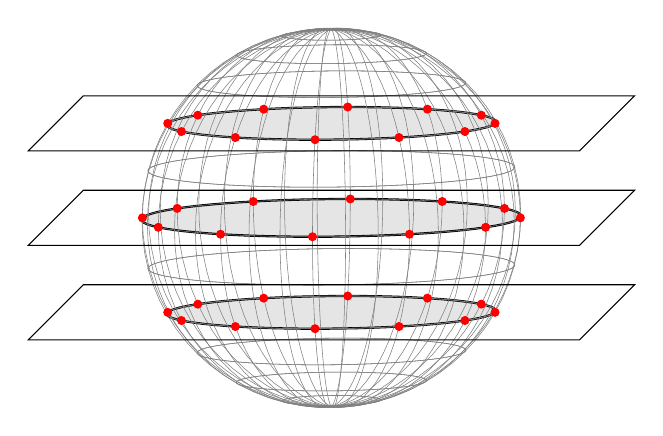
\begin{tikzpicture}
[
        n/.style={circle,fill=black,draw,inner sep=1pt},
x={(1cm,0)},y={(-1.0mm,-1.0mm)},z={(0,1cm)},
      ]

      \node[n] at (0,0,0) {};

      \def\r{2.4}


\foreach \h in {0,1.2,-1.2}{
        \pgfmathparse{sqrt(\r*\r-\h*\h)}
        \let\rr\pgfmathresult
        \filldraw[thick,fill=black!10] ({\rr*cos(0)},{\rr*sin(0)},\h)
        \foreach \t in {5,10,...,355}{
          -- ({\rr*cos(\t)},{\rr*sin(\t)},\h)
        } -- cycle;
      }

      \foreach \a in {0,10,...,170}{
        \draw[gray,very thin] ({\r*cos(\a)},{\r*sin(\a)},0)
        \foreach \t in {5,10,...,355}{
          -- ({\r*cos(\t)*cos(\a)},{\r*cos(\t)*sin(\a)},{\r*sin(\t)})
        } -- cycle;
      }

      \foreach \a in {-165,-150,...,165}{
        \pgfmathparse{sin(\a)*\r}
        \let\h\pgfmathresult
        \pgfmathparse{sqrt(\r*\r-\h*\h)}
        \let\rr\pgfmathresult
        \draw[gray,very thin] ({\rr*cos(0)},{\rr*sin(0)},\h)
        \foreach \t in {5,10,...,355}{
          -- ({\rr*cos(\t)},{\rr*sin(\t)},\h)
        } -- cycle;
      }

      \foreach \h in {0,1.2,-1.2}{
        \pgfmathparse{sqrt(\r*\r-\h*\h)}
        \let\rr\pgfmathresult
        \draw (-3.5,-3.5,\h) -- (-3.5,3.5,\h) -- (3.5,3.5,\h) -- (3.5,-3.5,\h) -- cycle;
        \foreach \t in {0,30,...,330}{
          \node[n,red] at ({\rr*cos(\t)},{\rr*sin(\t)},\h) {};
        }
      }

    \end{tikzpicture}
  \end{center}
  \vspace*{-12pt}
  \caption{Sphere cut with equidistant planes. Red points are the \emph{cluster positions}.}
  \label{sphere_fig}
\end{figure}
 
In addition, we also have the following.

\begin{corollary}
\label{sphere_thm_2}
Let  be a planar graph of degree . There is a 3D straight-line
drawing of  with an angular resolution of , with the vertices
of  placed on the surface of a sphere.
\end{corollary}
\begin{proof}
The proof
is a direct consequence of applying the algorithm from the proof of
Theorem~\ref{sphere_thm_2} and the fact that the degree of ,
the square of a planar graph, ,
has degree  \cite{DBLP:conf/focs/FormannHHKLSWW90}.
\qed
\end{proof}

Thus, we can produce 3D arc diagram drawings 
of planar graphs that achieve an angular resolution that is within a constant
factor of optimal. Admittedly, this type of drawing is probably
not going to be very pretty when rendered, say, as a video fly-through
on a 2D screen, as this type of drawing
is unlikely to project to a planar drawing in any direction.

\subsection{Stationary Vertices}
In this subsection, we show how to overcome the drawback of the above method,
in that we show how to start with any existing 2D straight-line drawing
and dramatically
improve the angular resolution for that drawing using a 3D arc diagram
rendering that projects perpendicularly to the 2D drawing.

\begin{theorem}
Let  be a straight-line drawing of a graph, , with arbitrary, but
distinct, placements for its vertices in the base plane.
There is a 3D arc diagram drawing of  with the same vertex
placements as  and with an angular resolution at least
, where  is the degree of ,
regardless of the angular resolution of .
\label{stationary_thm_1}
\end{theorem}
\begin{proof}
Since we are not allowed to move vertices, and edges have to lie
on planes perpendicular to the \emph{base plane}, we are restricted
to selecting angles  for edges  of . We do it by
utilizing classical edge coloring, observing that the ``entry''
and ``exit'' angles for each vertex need to match.

First, we compute an edge
coloring  of  with  colors ().
Then, for each edge , if its color in  is 
(), we set its angle to be
.
For any two edges , , the difference between their
angles  and 
is at least  (let ;
consider the plane, , determined by both tangent lines
having angle ; the angle between  and the plane
, on which tangent of  lies, is
).
Therefore, by Lemma~\ref{angle_lemma_2},
the angle between  and  in the arc diagram is also at least
.

It is unlikely that any pairs of the arcs touch each other in 3D, but
if any pair of them do touch, we can perturb one of them slightly to
eliminate the crossing, while still keeping the angular separation for
every pair of incident edges to be .
\qed
\end{proof}

In addition, through the use of a slanted 3D arc diagram rendering, we
can produce a drawing with angular resolution that is within a constant
factor of optimal, with each arc projecting to its corresponding 
straight-line edge in some direction.

\begin{theorem}
\label{stationary_vertices_thm_2}
Let  be a straight-line drawing of a graph, , 
with arbitrary, but distinct,
placements for its vertices in the base plane. There is a slanted 3D arc
diagram drawing of  with the same vertex placements as  and
with an angular resolution at least , where  is the
degree of , regardless of the angular resolution of .
\end{theorem}

\begin{proof}
Let  be a set of  uniformly distributed
angles from  to . Define a set of  ``colors'' as distinct
pairs, , where  and  are each in .
Compute an edge coloring of  using these colors. Now let  be an edge
in , which is colored with . Draw the edge, , using
a circular arc that lies in a plane, , that makes an angle of
 with the \emph{base plane} and
which has a tangent in  that forms an angle of  at each
endpoint of .
(For instance, in Fig.~\ref{fig:3darcs}b,
we give a slanted 3D arc diagram based on the edge coloring of the graph
in Fig.~\ref{fig:3darcs}a, corresponding to the following 
    (, ) ``colors:''
    \textcolor{blue}{(0, 0)},
    \textcolor{magenta}{(, 0)},
    \textcolor{Sepia}{(, 0)},
    \textcolor{orange}{(, 22.5)},
    \textcolor{green}{(, 45)}.)

The claim is that every pair of incident edges is separated by an
angle of size at least . So suppose  and  are
two edges incident on the same vertex, .  Let 
be the color of  and let  be the color of .
Since  and  are incident and we computed a valid coloring for
,  or . In either
case, this implies that  and  are separated by an angle of size
at least  (by Lemma~\ref{angle_lemma_1} if
, by Lemma~\ref{angle_lemma_2} otherwise),
which establishes the claim.
As previously, we can perturb the arcs to eliminate crossings in 3D.
\qed
\end{proof}

Thus, we can achieve optimal angular resolution in a 3D arc diagram
for any graph, , to within a constant factor, for any arbitrary
placement of vertices of  in the plane. Note, however, that even if
 is planar, the 3D arc diagram this algorithm produces,
when projected to the \emph{base plane}, may create edge crossings in the
projected drawing.  It would be nice, therefore, to have 3D arc
diagrams that could have good angular resolution and also have planar
perpendicular projections in the \emph{base plane}.

\subsection{Free Vertices}
In this section, we show how to take any 2D straight-line 
drawing with good angular resolution and convert it to a 3D arc diagram
with angular resolution that is within a constant factor of optimal.
Moreover, this is the result that makes use of a localized edge coloring.

\begin{theorem}
Let  be a straight-line drawing of a graph, , with arbitrary,
but distinct, placement for its vertices in the base plane, and
 angular resolution. There is
a 3D arc diagram drawing of  with the same vertex placements as 
and with angular resolution at least , where 
is the degree of , such that all arcs project perpendicularly
as straight lines onto the base plane.
\label{free_vertices_thm}
\end{theorem}
\begin{proof}
The algorithm is similar to the one from the proof of
Theorem~\ref{stationary_thm_1}. This time, however, we first compute an
-localized edge coloring, , of  utilizing  colors
(). Then, as previously, we assign angle
 to an edge  of color  in
 ().

Let us consider two arcs,  and , incident on a vertex, .
If , then the angle between  and 
is at least , by Lemma~\ref{angle_lemma_2}.
Otherwise, , and  and  have the same
color in . By the definition of -localized edge
coloring,  and  are separated by at least  edges around
. Because  has resolution , the angle
between  and  in  is . Thus, by
Lemma~\ref{angle_lemma_1}, the angle between  and 
is also .
Therefore, the angle between  and  is
. We achieve the
advertised angular resolution by setting .
\qed
\end{proof}

Theorem~\ref{free_vertices_thm} shows that we can achieve
 angular resolution in a 3D arc diagram drawing
of a graph, , with arcs projecting perpendicularly onto the base plane
as straight-line segments, if there is a straight-line drawing of 
on a plane with an angular resolution of . The following is
an immediate consequence.

\begin{corollary}
There is a 3D arc diagram drawing of any planar graph, ,
with straight-line projection onto the base plane,
and an angular resolution of .
\end{corollary}
\begin{proof}
By~\cite{DBLP:conf/focs/FormannHHKLSWW90}, we can draw 
in a straight-line manner on a plane with an angular
resolution of .
\qed
\end{proof}

Admittedly, the 2D projection of this graph is not necessarily planar.
We can nevertheless also achieve the following.

\begin{corollary}
There is a 3D arc diagram drawing of any ordered tree, ,
with straight-line projection onto the base plane,
and an angular resolution of .
\end{corollary}
\begin{proof}
By Duncan {\it et al.}~\cite{degkn-dtp-11},
we can draw 
in a straight-line manner on a plane with an angular resolution of .
\qed
\end{proof}

In addition, the area of the projection of the drawings produced by the
previous two corollaries is polynomial.

